% verso e anverso:
% \documentclass[12pt,openright,twoside,a4paper,english]{abntex2}
% apenas verso:	
\documentclass[12pt,oneside,a4paper,english]{abntex2} 

\usepackage[alf]{abntex2cite}	% Citações padrão ABNT
\usepackage{listings}
\usepackage{float}
\usepackage{cmap}				% Mapear caracteres especiais no PDF
\usepackage{lmodern}			% Usa a fonte Latin Modern			
\usepackage[T1]{fontenc}		% Selecao de codigos de fonte.
\usepackage[utf8]{inputenc}		% Codificacao do documento (conversão automática dos acentos)
\usepackage{lastpage}			% Usado pela Ficha catalográfica
\usepackage{indentfirst}		% Indenta o primeiro parágrafo de cada seção.
\usepackage{color}				% Controle das cores
\usepackage{graphicx}			% Inclusão de gráficos
\usepackage{pdfpages}
\usepackage{tikz}
\usetikzlibrary{automata,positioning}

\definecolor{blue}{RGB}{41,5,195} % alterando o aspecto da cor azul

\makeatletter
\hypersetup{
    %pagebackref=true,
    pdftitle={\@title}, 
    pdfauthor={\@author},
    pdfsubject={\@title},
    pdfcreator={\imprimirpreambulo},
    pdfkeywords={Linguagens}{Compiladores}{Analisador Léxico}, 
    colorlinks=true,       		% false: boxed links; true: colored links
    linkcolor=blue,          	% color of internal links
    citecolor=blue,        		% color of links to bibliography
    filecolor=magenta,      		% color of file links
    urlcolor=blue,
    bookmarksdepth=4
}
\makeatother

\autor{Gustavo P. Gouveia (6482819), Victor Lassance (6431325)}
\title{Relatório de Compiladores - Primeira Etapa - Construção de um analisador léxico}
\orientador[Professor:]{Ricardo Luis de Azevedo da Rocha}
\preambulo{Texto apresentado à Escola Politécnica da Universidade de São Paulo como requisito para a aprovação na disciplina Linguagens e Compiladores no quinto módulo acadêmico do curso de graduação em Engenharia de Computação, junto ao Departamento de Engenharia de Computação e Sistemas Digitais (PCS).}
\instituicao{%
	Universidade de São Paulo
	\par
	Escola Politécnica
	\par
	Engenharia de Computação - Curso Cooperativo}
\local{São Paulo}
\data{2013}
\tipotrabalho{PCS2056 - Linguagens e Compiladores}

\setlength{\parindent}{1.3cm} % O tamanho do parágrafo
\setlength{\parskip}{0.2cm}  % Controle do espaçamento entre um parágrafo e outro

\makeindex

\begin{document}

\frenchspacing % Retira espaço extra obsoleto entre as frases.

\imprimircapa
\imprimirfolhaderosto

\clearpage
\begin{resumo}
	% !TEX encoding = UTF-8 Unicode
Este trabalho descreve a concepção e o desenvolvimento de um compilador utilizando a linguagem C. O escopo do compilador se limita a casos mais simples, porém simbólicos, e que servem ao aprendizado do processo de criação e teste de um compilador completo. A estrutura da linguagem escolhida para ser implementada se assemelha a própria estrutura do C, por facilidade de compreensão.

\vspace{\onelineskip}
    
\noindent
\textbf{Palavras-chaves}: Linguagens, Compiladores, Analisador Léxico.

\end{resumo}

\tableofcontents

\textual

\chapter{Introdução}
\label{chap:introducao}
	% !TEX encoding = UTF-8 Unicode

Este projeto tem como objetivo a construção de um compilador de um só passo, dirigido por sintaxe, com analisador e reconhecedor sintático baseado em autômato de pilha estruturado.

Em um primeiro momento, foi definida uma linguagem de programação e identificados os tipos de átomos. Para cada átomo foi escrito uma gramática linear representativa da sua lei de formação e um reconhecedor para o átomo. Desse modo, as gramáticas assim escritas foram unidas e convertidas em um autômato finito, o qual foi transformado em um transdutor e implementado como sub-rotina, dando origem ao analisador léxico propriamente dito. Também foi criada uma função principal para chamar o analisador léxico e possibilitar o seu teste.

Durante a segunda etapa, a sintaxe da linguagem, denonimada por nós de CZAR, foi definida formalmente a partir de uma definição informal e de exemplos de programas que criamos, misturando palavras-chave e conceitos de diferentes linguagens de programação. As três principais definições foram escritas na notação BNF\footnote{Ver http://en.wikipedia.org/wiki/Backus\_Naur\_Form}, Wirth\footnote{Ver http://en.wikipedia.org/wiki/Wirth\_syntax\_notation} e com diagramas de sintaxe.

Na terceira etapa, implementamos o módulo referente à parte sintática para a nossa linguagem. O analisador sintático construído obtém uma cadeia de \emph{tokens} proveniente do analisador léxico, e verifica se a mesma pode ser gerada pela gramática da linguagem e, com isso, constrói a árvore sintática \cite{alfred1986compilers}.

Para a quarta entrega, focamos no ambiente de execução. O compilador por nós criado tem como linguagem de saída um programa que é executado na máquina virtual conhecida como Máquina de von Neumann (MVN).

Já durante as duas últimas entregas, complementamos a especificação do código gerado pelo compilador e das rotinas do ambiente de execução da nossa linguagem de alto nível, a CZAR. Além disso, buscamos integrar as rotinas semânticas no reconhecedor sintático de forma a permitir a geração de código e finalizar o compilador.

Como material de consulta, além de sites sobre o assunto e das aulas ministradas, foi utilizado o livro indicado pelo professor no começo das aulas \cite{intro-compiladores}, para pesquisa de conceitos e possíveis implementações.

O documento apresenta a seguir o processo completo de desenvolvimento de um compilador, desde a definição formal da linguagem, passando pelo analisador léxico, reconhecedor sintático, pela definição do ambiente de execução e das rotinas semânticas, terminando com um exemplo de programa traduzido.


\chapter{Questões}
\label{chap:questoes}
	% !TEX encoding = UTF-8 Unicode

A seguir, seguem as respostas às questões propostas pelo professor.

\section{Questão 1}
\label{chap:q1}
	% !TEX encoding = UTF-8 Unicode

\textbf{Quais são as funções do analisador léxico nos compiladores e interpretadores?}

TODO


\section{Questão 2}
\label{chap:q2}
	% !TEX encoding = UTF-8 Unicode

\textbf{Quais as vantagens e desvantagens da implementação do analisador léxico como uma fase separada do processamento da linguagem de programação em relação à sua implementação como sub-rotina que vai extraindo um átomo a cada chamada?}

TODO

	
\section{Questão 3}
\label{chap:q3}
	% !TEX encoding = UTF-8 Unicode

\textbf{Defina formalmente, através de expressões regulares sobre o conjunto de caracteres ASCII, a sintaxe de cada um dos tipos de átomos a serem extraídos do texto-fonte pelo analisador léxico, bem como de cada um dos espaçadores e comentários.}

TODO


\section{Questão 4}
\label{chap:q4}
	% !TEX encoding = UTF-8 Unicode

\textbf{Converta cada uma das expressões regulares, assim obtidas, em autômatos finitos equivalentes que reconheçam as correspondentes linguagens por elas definidas.}

\begin{itemize}

\item DELIM: \verb!/[{}()\[\];]/!

\begin{figure}[H]
	\centering
	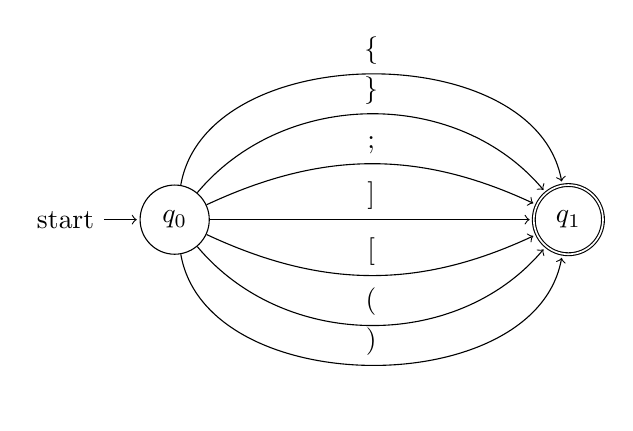
\begin{tikzpicture}[shorten >=1pt,node distance=5cm,on grid,auto] 
	   \node[state,initial] (q0)   {$q_0$}; 
	   \node[state,accepting](q1) [right=of q0] {$q_1$};
	    \path[->] 
	    (q0) edge[bend left=80]   node {\{} (q1)
	    (q0) edge[bend left=50]   node {\}} (q1)
	    (q0) edge[bend right=50]  node {(} (q1)
	    (q0) edge[bend right=80]  node {)} (q1)
	    (q0) edge[bend left=25]   node {;} (q1)
	    (q0) edge[bend right=25]  node {[} (q1)
	    (q0) edge                 node {]} (q1);
	\end{tikzpicture}
	\caption{Autômato finito DELIM}
\end{figure}

\item SPACE: \verb!/[ \t\r\n\v\f]+/!

\begin{figure}[H]
	\centering
	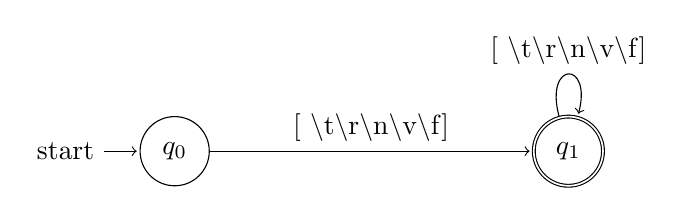
\begin{tikzpicture}[shorten >=1pt,node distance=5cm,on grid,auto] 
	   \node[state,initial] (q0)   {$q_0$}; 
	   \node[state,accepting](q1) [right=of q0] {$q_1$};
	    \path[->] 
	    (q0) edge   node {
			[ $\backslash$t$\backslash$r$\backslash$n$\backslash$v$\backslash$f]
		} (q1)
		(q1) edge[loop above]  node {
			[ $\backslash$t$\backslash$r$\backslash$n$\backslash$v$\backslash$f]
		} (q1);
	\end{tikzpicture}
	\caption{Autômato finito SPACE}
\end{figure}

\item COMMENT: \verb!/#[^\n]*/!

\begin{figure}[H]
	\centering
	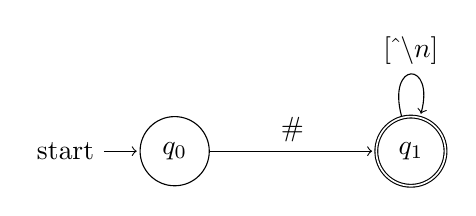
\begin{tikzpicture}[shorten >=1pt,node distance=3cm,on grid,auto] 
	   \node[state,initial] (q0)   {$q_0$}; 
	   \node[state,accepting](q1) [right=of q0] {$q_1$};
	    \path[->] 
	    (q0) edge  node {\#} (q1)
		(q1) edge[loop above]  node {$[\hat{~}\backslash n]$} (q1);
	\end{tikzpicture}
	\caption{Autômato finito COMMENT}
\end{figure}

\item IDENT: \verb!/[a-zA-Z_][a-zA-Z0-9_]*/!

\begin{figure}[H]
	\centering
	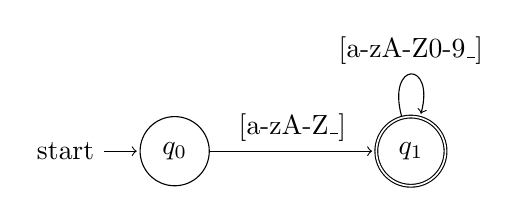
\begin{tikzpicture}[shorten >=1pt,node distance=3cm,on grid,auto] 
	   \node[state,initial] (q0)   {$q_0$}; 
	   \node[state,accepting](q1) [right=of q0] {$q_1$};
	    \path[->] 
	    (q0) edge  node {[a-zA-Z\_]} (q1)
	    (q1) edge [loop above] node {[a-zA-Z0-9\_]} (q1);
	\end{tikzpicture}
	\caption{Autômato finito IDENT}
\end{figure}

\item INTEGER: \verb!/[0-9]+/!

\begin{figure}[H]
	\centering
	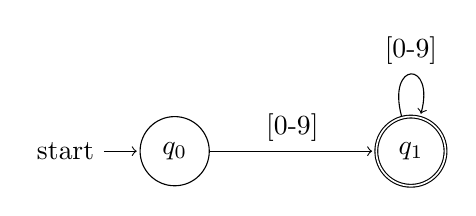
\begin{tikzpicture}[shorten >=1pt,node distance=3cm,on grid,auto] 
	   \node[state,initial] (q0)   {$q_0$}; 
	   \node[state,accepting](q1) [right=of q0] {$q_1$};
	    \path[->] 
	    (q0) edge  node {[0-9]} (q1)
	    (q1) edge [loop above] node {[0-9]} (q1);
	\end{tikzpicture}
	\caption{Autômato finito INTEGER}
\end{figure}

\item FLOAT: \verb!/[0-9]*\.[0-9]+/!

\begin{figure}[H]
	\centering
	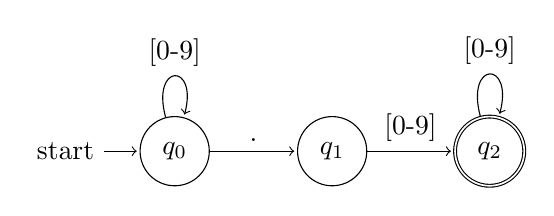
\begin{tikzpicture}[shorten >=1pt,node distance=2cm,on grid,auto] 
	   \node[state,initial] (q0)   {$q_0$}; 
	   \node[state](q1) [right=of q0] {$q_1$};
	   \node[state,accepting](q2) [right=of q1] {$q_2$};
	    \path[->] 
	    (q0) edge  node {.} (q1)
	    (q1) edge  node {[0-9]} (q2)
	    (q0) edge [loop above] node {[0-9]} (q0)
	    (q2) edge [loop above] node {[0-9]} (q2);
	\end{tikzpicture}
	\caption{Autômato finito FLOAT}
\end{figure}

\item CHAR: \verb!/'(?:\\[abtnvfre\\]|[\x20-\x5B\x5D-\x7E])?'/!

\begin{figure}[H]
	\centering
	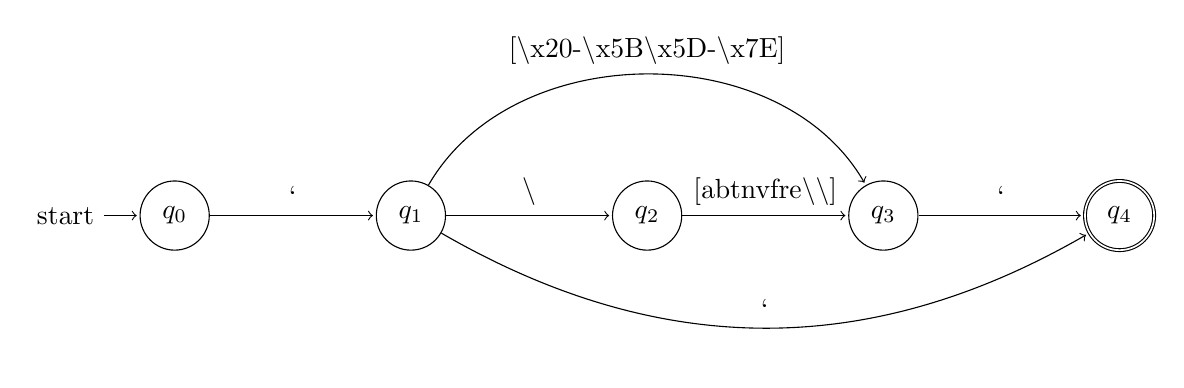
\begin{tikzpicture}[shorten >=1pt,node distance=3cm,on grid,auto] 
	   \node[state,initial] (q0)   {$q_0$}; 
	   \node[state] (q1) [right=of q0] {$q_1$}; 
	   \node[state] (q2) [right=of q1] {$q_2$}; 
	   \node[state] (q3) [right=of q2] {$q_3$}; 
	   \node[state, accepting] (q4) [right=of q3] {$q_4$}; 
	    \path[->] 
	    (q0) edge  node {$`$} (q1)
	    (q1) edge[bend left=60] node {
	        [$\backslash$x20-$\backslash$x5B$\backslash$x5D-$\backslash$x7E]
	    } (q3)
	    (q1) edge node {$\backslash$} (q2)
	    (q2) edge node {[abtnvfre$\backslash\backslash$]} (q3)
	    (q3) edge node {$`$} (q4)
		(q1) edge[bend right=30] node {$`$} (q4);
	\end{tikzpicture}
	\caption{Autômato finito CHAR}
\end{figure}

\item STRING: \verb!/"(?:\\"|[^"])*"/!

\begin{figure}[H]
	\centering
	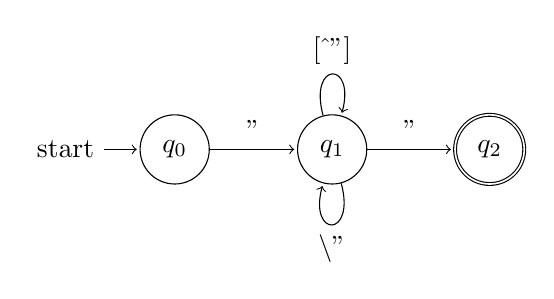
\begin{tikzpicture}[shorten >=1pt,node distance=2cm,on grid,auto] 
	   \node[state,initial] (q0)   {$q_0$}; 
	   \node[state] (q1) [right=of q0] {$q_1$}; 
	   \node[state, accepting] (q2) [right=of q1] {$q_2$}; 
	    \path[->] 
	    (q0) edge  node {$"$} (q1)
	    (q1) edge [loop above] node {$[\hat{~}"]$} (q1)
	         edge [loop below] node {$\backslash"$} (q1)

	    (q1) edge  node {$"$} (q2);
	\end{tikzpicture}
	\caption{Autômato finito STRING}
\end{figure}

\item OPER: \verb$/[\+\-\*\/%=!<>][=]?/$

\begin{figure}[H]
	\centering
	\begin{tikzpicture}[shorten >=1pt,node distance=7cm,on grid,auto] 
		\centering
	    \node[state,initial] (q0)   {$q_0$}; 
	    \node[state,accepting](q1) [right=of q0] {$q_1$};
	    \node[state,accepting](q2) [right=of q2] {$q_2$};
	    \path[->] 
	    (q0) edge   node {$+$} (q1)
	    (q0) edge[bend right=65]  node {$-$} (q1)
	    (q0) edge[bend left=65]   node {$*$} (q1)
	    (q0) edge[bend right=45]  node {$/$} (q1)
	    (q0) edge[bend left=45]   node {$\%$} (q1)
	    (q0) edge[bend right=30]  node {$!$} (q1)
	    (q0) edge[bend left=30]   node {$<$} (q1)
	    (q0) edge[bend left=15]   node {$>$} (q1)
	    (q0) edge[bend right=15]  node {$=$} (q1)
	    (q1) edge   node {$=$} (q2);
	\end{tikzpicture}
	\caption{Autômato finito OPER}
\end{figure}

\end{itemize}

\section{Questão 5}
\label{chap:q5}
	% !TEX encoding = UTF-8 Unicode

\textbf{Crie um autômato único que aceite todas essas linguagens a partir de um mesmo estado inicial, mas que apresente um estado final diferenciado para cada uma delas.}

    
\begin{itemize}
    \item C\_DELIM $= [91, 93, 123, 125, 40, 41, 59]$
    \item C\_SPACE $= [32, 9, 10, 11, 12, 13]$
    \item C\_OPER  $= [42, 37, 60, 62, 43, 61, 33, 47, 45]$
    \item C\_LETTERS  $= [65, \dots, 90, 97, \dots, 122, 95]$
    \item C\_NUMBERS  $= [48, 57]$ 
\end{itemize}
\resizebox{400px}{400px}{
    \centering
\begin{tikzpicture}[shorten >=1pt,node distance=5cm,on grid,auto] 


    \node[state,initial] (q0)   {$q_0$}; 
    \node[state,accepting](delim) [right=of q0, yshift=130, xshift=-100] {delim};
    \node[state](comm) [right=of q0, yshift=100, xshift=-210] {comm};
    \node[state,accepting](comm2) [above=of comm, yshift=-30] {$comm_2$};
    \node[state,accepting](space) [right=of q0, yshift=100, xshift=20] {space};
    \node[state,accepting](oper) [right=of q0, yshift=20, xshift=40] {oper};
    \node[state,accepting](oper2) [right=of oper] {$oper_2$};
    \node[state,accepting](ident) [right=of q0, yshift=-30, xshift=40] {$ident$};
    \node[state,accepting](ident2) [right=of ident] {$ident_2$};
    \node[state,accepting](integ) [right=of q0, yshift=-100, xshift=-100] {$int$};
    \node[state](float) [right=of integ, xshift=20] {$float$};
    \node[state,accepting](float2) [right=of float] {$float_2$};
    \node[state] (char1) [left=of q0, yshift=-60] {$char$}; 
    \node[state] (char2) [below=of char1] {$char_2$}; 
    \node[state] (char3) [below=of char2] {$char_3$}; 
    \node[state, accepting] (char4) [right=of char3] {$char_4$}; 
    \node[state] (str1) [left=of q0, yshift=60] {$str_1$}; 
    \node[state, accepting] (str2) [above=of str1] {$str_2$};
    \path[->] 

    (q0) edge node {$\$$} (comm)
    (comm) edge [loop left] node {$[\hat{~}\backslash{}n]$} (comm)
    (comm) edge node {$\backslash{}n$} (comm2)
    (q0) edge node {C\_DELIM} (delim)
    (q0) edge node {C\_SPACE} (space)
    (q0) edge node {C\_OPER} (oper)
    (oper) edge node {$=$} (oper2)
    (q0) edge node {C\_LETTERS} (ident)
    (ident) edge [bend left=19] node {C\_LETTERS $|$ C\_NUMBERS} (ident2)
    (q0) edge [bend right=19] node {C\_NUMBERS} (integ)
    (integ) edge [loop below] node {C\_NUMBERS} (integ)
    (q0) edge  [bend left=19] node {$.$} (float)
    (integ) edge node {$.$} (float)
    (float) edge  node {C\_NUMBERS} (float2)
    (float2) edge [loop below] node {C\_NUMBERS} (float2)
    (q0) edge  node {$'$} (char1)
    (char1) edge[bend left=60] node { %
        [$\backslash$x20-$\backslash$x5B$\backslash$x5D-$\backslash$x7E] %
    } (char3) 
    (char1) edge node {$\backslash$} (char2)
    (char2) edge node {[abtnvfre$\backslash\backslash$]} (char3)
    (char3) edge  node {$'$} (char4)
    (q0) edge  node {$"$} (str1)
    (str1) edge [loop left] node {$[\hat{~}"]$} (str1)
           edge [loop right] node {$\backslash"$} (str1)
           edge  node {$"$} (str2);
\end{tikzpicture}
}


\section{Questão 6}
\label{chap:q6}
	% !TEX encoding = UTF-8 Unicode

\textbf{Transforme o autômato assim obtido em um transdutor, que emita como saída o átomo encontrado ao abandonar cada um dos estados finais para iniciar o reconhecimento de mais um átomo do texto.}

O transdutor obtido a partir da transformação da questão 5 pode ser encontrado no apêndice \ref{app:transdutor}.


\section{Questão 7}
\label{chap:q7}
	% !TEX encoding = UTF-8 Unicode

\textbf{Converta o transdutor assim obtido em uma sub-rotina, escrita na linguagem de programação de sua preferência.}

A sub-rotina escrita e testada pode ser encontrada no apêndice \ref{app:codigo-lexico}.
O código está comentado e seu funcionamento é explicado na questão 9.


\section{Questão 8}
\label{chap:q8}
	% !TEX encoding = UTF-8 Unicode

\textbf{Crie um programa principal que chame repetidamente a sub-rotina assim construída, e a aplique sobre um arquivo do tipo texto contendo o texto-fonte a ser analisado. Após cada chamada, esse programa principal deve imprimir as duas componentes do átomo extraído (o tipo e o valor do átomo encontrado).}

TODO


\section{Questão 9}
\label{chap:q9}
	% !TEX encoding = UTF-8 Unicode

\textbf{Relate detalhadamente o funcionamento do analisador léxico assim construído, incluindo no relatório: descrição teórica do programa; descrição da sua estrutura; descrição de seu funcionamento; descrição dos testes realizados e das saídas obtidas.}

TODO


\section{Questão 10}
\label{chap:q10}
	% !TEX encoding = UTF-8 Unicode

\textbf{Explique como enriquecer esse analisador léxico com um expansor de macros do tipo \#DEFINE, não paramétrico nem recursivo, mas que permita a qualquer macro chamar outras macros, de forma não cíclica.}

TODO



\chapter{Exemplo de Execução}
\label{chap:execucao}
	% !TEX encoding = UTF-8 Unicode

Um código de exemplo que foi utilizado para teste está listado abaixo:

\textbf{\emph{ENTRADA.txt}}
\lstinputlisting[frame=single,language=C,numbers=left,breaklines=true]{ENTRADA.txt}

Ao utilizar o código acima como \emph{input}, obtivemos o seguinte resultado, que foi de acordo com o esperado:

\textbf{\emph{Resultado sem erros}}
\lstinputlisting[frame=single,numbers=left,breaklines=true]{testes/Resultado_sem_erros.txt}

Ao introduzir um erro colocando mais de uma letra como caracter, obtivemos, como esperado, o seguinte resultado:

\textbf{\emph{Resultado com erro}}
\lstinputlisting[frame=single,numbers=left,breaklines=true]{testes/Resultado_com_erro.txt}


\chapter{Considerações Finais}
\label{chap:conclusao}
	% !TEX encoding = UTF-8 Unicode

O projeto do compilador é um projeto muito interessante, porém complexo. Desta forma, a divisão em etapas bem estruturadas permite o aprendizado e teste de cada uma das etapas. Nesse primeiro momento, o foco foi no analisador léxico, o que permitiu realizar o \emph{parse} do código e transformá-lo em tokens. Para a realização do analisador, tentamos pensar em permitir o processamento das principais classes de tokens, com o intuito de entender o funcionamento de um compilador de forma prática e didática.

Para as próximas etapas, espera-se atualizar o analisador léxico quando for necessário, visando agregar os ensinamentos das próximas aulas.


\bibliography{bibliografia}

\begin{apendicesenv} % Inicia os apêndices

% Imprime uma página indicando o início dos apêndices
\partapendices

\chapter{Transdutor do Analisador Léxico}
\label{app:transdutor}
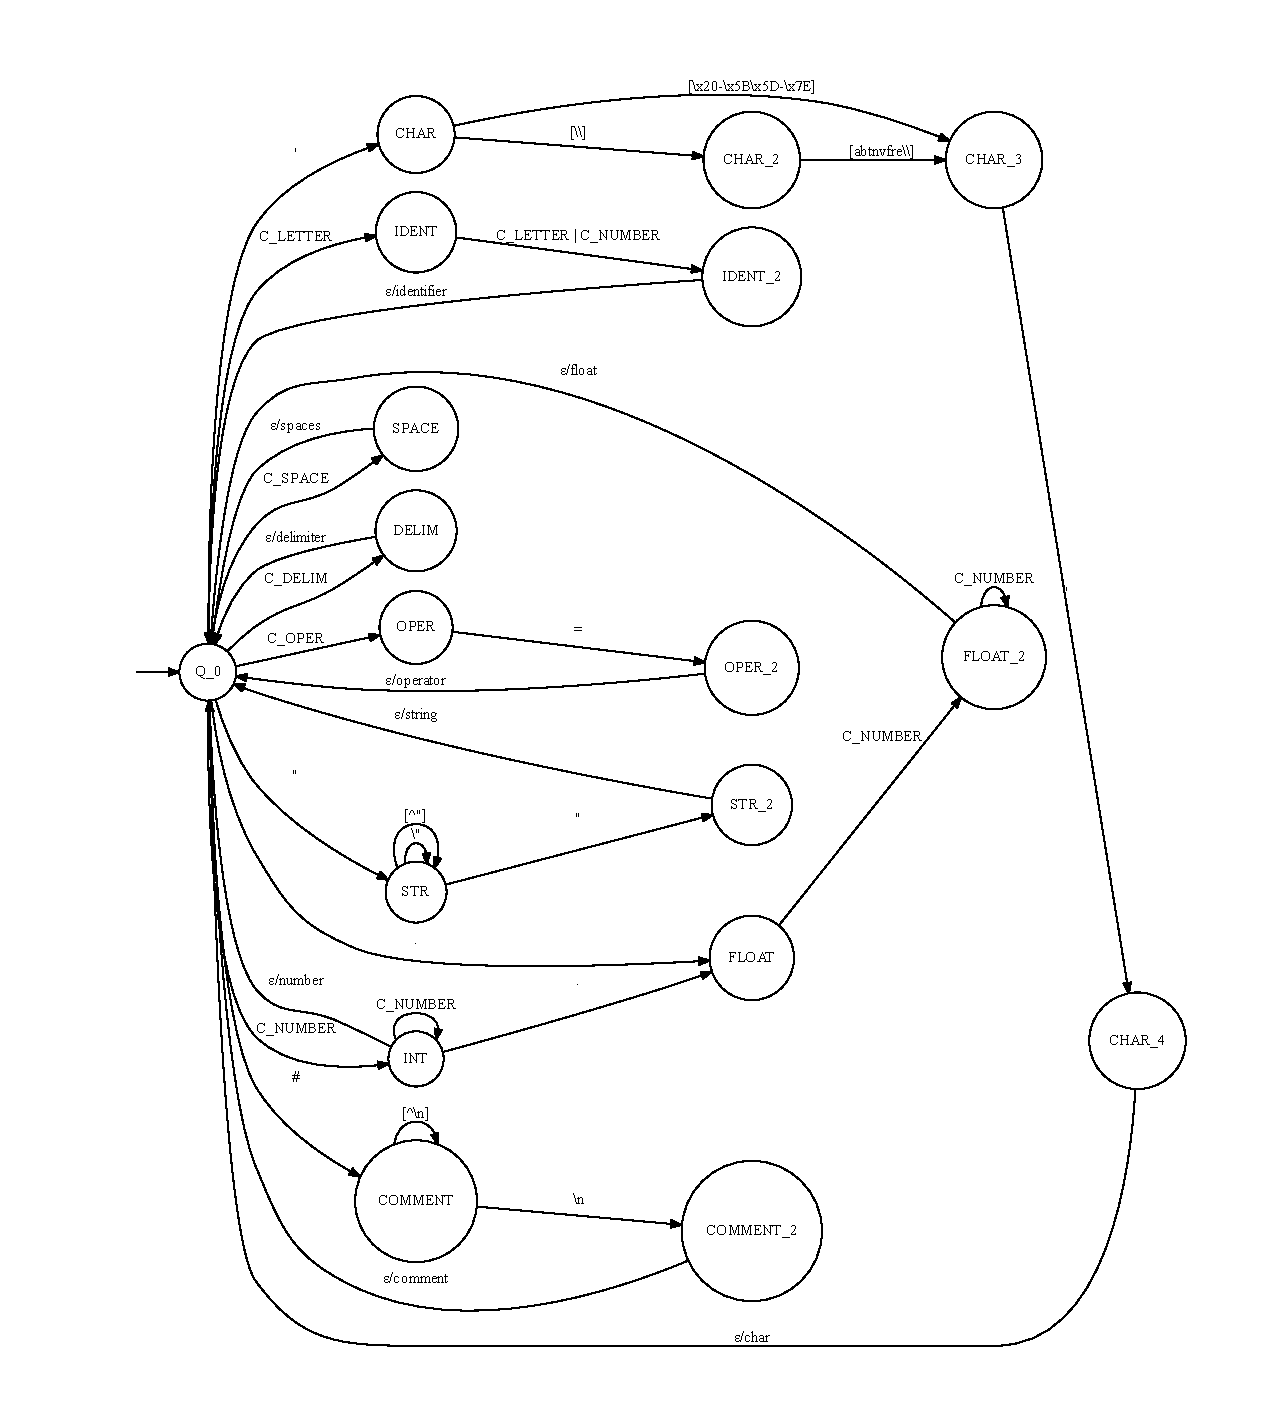
\includepdf[pages={1}]{automatos/transdutor.pdf}

\chapter{Código em C da sub-rotina do Analisador Léxico}
\label{app:codigo-lexico}
\textbf{\emph{lex.h}}
\lstinputlisting[frame=single,language=C,numbers=left,breaklines=true]{../lex/lex.h}
\textbf{\emph{lex.c}}
\lstinputlisting[frame=single,language=C,numbers=left,breaklines=true]{../lex/lex.c}

\chapter{Código em C do método principal do Analisador Léxico}
\label{app:codigo-principal}
\lstinputlisting[frame=single,language=C,numbers=left,breaklines=true]{../lex/test.c}

\end{apendicesenv}

\end{document}
